LLVM代码生成器接受IR中描述的模块作为输入,并将其转换为目标代码或汇编文本,我们需要将AST表示转换为IR。为了实现IR代码生成器,我们将首先查看一个简单的示例,然后开发代码生成器所需的类。完整的实现将分为三个类:CodeGenerator、CGModule和CGProcedure类。CodeGenerator类是编译器驱动程序使用的通用接口。CGModule和CGProcedure类保存了为编译单元和单个函数生成IR代码所需的状态。\par

下一节中,我们首先看看Clang生成的IR。\par


\hspace*{\fill} \par %插入空行
\textbf{了解IR代码}

生成IR代码之前,最好先了解IR语言的主要元素。在第3章中,我们已经简要地了解了IR。获得更多IR的一个简单方法是研究clang的输出。例如,保存以下C源代码,它实现了计算两个数的最大公约数的欧几里得算法:\par

\begin{lstlisting}[caption={}]
unsigned gcd(unsigned a, unsigned b) {
	if (b == 0)
	return a;
	while (b != 0) {
		unsigned t = a % b;
		a = b;
		b = t;
	}
	return a;
}
\end{lstlisting}

然后可以使用以下命令,创建IR文件gcd.ll:\par

\begin{tcolorbox}[colback=white,colframe=black]
\$ clang --target=aarch64-linux-gnu –O1 -S -emit-llvm gcd.c
\end{tcolorbox}

IR代码与目标有关,该命令用于编译Linux环境下ARM 64位CPU的源文件。-S选项指示clang输出一个程序集文件,通过附加的-emit-llvm,创建一个IR文件。优化级别-O1用于获得易读的IR代码。看一下生成的文件,并理解C源代码如何映射到IR。在文件的顶部,有一些基本信息:\par

\begin{tcolorbox}[colback=white,colframe=black]
; ModuleID = 'gcd.c' \\
source\underline{~}filename = "gcd.c" \\
target datalayout = "e-m:e-i8:8:32-i16:16:32-i64:64- \\
\hspace*{3.5cm}i128:128-n32:64-S128" \\
target triple = "aarch64-unknown-linux-gnu"
\end{tcolorbox}

第一行是注释,说明使用了哪个模块标识符。下一行中,注明了源文件的文件名。对于clang,两者一样。\par

target datalayout字符串建立了一些基本属性。它的各个部分用-隔开。包括以下信息:\par

\begin{itemize}
\item 小e意味着内存中的字节使用小端模式存储。要指定大的端序,可以使用大写的E。
\item 指定应用于符号的名称转换。这里,m:e表示使用ELF名称mangling。
\item 在iN:A:P形式中的条目i8:8:32,指定了数据的对齐方式,以位为单位。第一个数字是ABI所需的对齐方式,第二个数字是首选的对齐方式。对于bytes (i8), ABI对齐是1字节(8),首选对齐是4字节(32)。
\item n指定可用的本机寄存器大小。n32:64意味着本地支持32位和64位宽整数。
\item s指定堆栈的对齐方式,同样以位为单位。S128表示堆栈保持16字节对齐。
\end{itemize}

\begin{tcolorbox}[colback=blue!5!white,colframe=blue!75!black,title=Note]
目标数据的更多的信息,你以在参考手册\url{https://llvm.org/docs/LangRef.html#data-layout}。
\end{tcolorbox}

最后,target triple字符串指定了我们要编译的体系结构。对于我们在命令行中给出的信息来说,这是必不可少的。这个在第2章,已经进行了深入的讨论。\par

接下来,在IR文件中定义gcd函数:\par

\begin{tcolorbox}[colback=white,colframe=black]
define i32 @gcd(i32 \%a, i32 \%b) \{
\end{tcolorbox}

这类似于C文件中的函数签名。unsigned数据类型被转换为32位整数类型i32。函数名以@作为前缀,参数名以\%作为前缀。函数体用大括号括起来。正文代码如下:\par

\begin{tcolorbox}[colback=white,colframe=black]
entry: \\
\hspace*{0.5cm}\%cmp = icmp eq i32 \%b, 0 \\
\hspace*{0.5cm}br i1 \%cmp, label \%return, label \%while.body
\end{tcolorbox}

IR代码组织在基本块中。结构良好的\textbf{基本块}是指令的线性序列,它以可选标签开始,以终止指令(例如,分支或返回指令)结束。因此,每个基本块都有一个入口点和一个出口点。LLVM允许在构造时出现畸形的基本块。第一个基本块的标签是entry。块中的代码很简单:第一个指令比较参数\%b和0。第二个指令分支到label return,如条件为真,则分支到label while;若条件为假,则返回.\par

IR代码的另一个特点是\textit{SSA}形式的。代码使用无限数量的虚拟寄存器,但每个寄存器只编写一次。比较的结果分配给指定的虚拟寄存器\%cmp。这个寄存器随后会使用,但它永远不会再写入。诸如常量传播和公共子表达式消除之类的优化在SSA表单中工作得非常好,所有现代编译器都在使用它。\par

下一个基本块是while的循环体:\par

\begin{tcolorbox}[colback=white,colframe=black]
while.body: \\
\hspace*{0.5cm}\%b.addr.010 = phi i32 [ \%rem, \%while.body ], \\
\hspace*{3.5cm}[ \%b, \%entry ] \\
\hspace*{0.5cm}\%a.addr.09 = phi i32 [ \%b.addr.010, \%while.body ], \\
\hspace*{3.5cm}[ \%a, \%entry ] \\
\hspace*{0.5cm}\%rem = urem i32 \%a.addr.09, \%b.addr.010 \\
\hspace*{0.5cm}\%cmp1 = icmp eq i32 \%rem, 0 \\
\hspace*{0.5cm}br i1 \%cmp1, label \%return, label \%while.body
\end{tcolorbox}

在gcd循环中,赋于a和b参数以新值。如果一个寄存器只能写入一次,那么是无法完成的。解决方法是使用特殊的phi指令,phi指令有一个基本块列表和值作为参数。一个基本块表示从哪边的基本块进入的,值就是那些基本块的值。在运行时,phi指令将前面执行的基本块的标签与参数列表中的标签进行比较。\par

指令的值与标签的值相关联。对于第一个phi指令,如果之前执行的基本块是while.body,则值为\%rem。如果entry是前面执行的基本块,则该值为\%b。这些值位于基本块的开始部分。\%b.addr.010从第一个phi指令中得到一个值。在第二个phi指令的参数列表中使用了相同的寄存器,但该值假定为通过第一个phi指令改变它之前的值。\par

在循环体之后,必须选择返回值:\par

\begin{tcolorbox}[colback=white,colframe=black]
return: \\
\hspace*{0.5cm}\%retval.0 = phi i32 [ \%a, \%entry ], \\
\hspace*{3.5cm}[ \%b.addr.010, \%while.body ] \\
\hspace*{0.5cm}ret i32 \%retval.0 \\
\}
\end{tcolorbox}

同样,使用phi指令来选择所需的值。ret指令不仅可以结束这个基本块,还表示该函数在运行时的结束。它将返回值作为参数。\par

对于phi指令的使用有一些限制,必须是基本块的第一个指令。第一个基本块是特殊的:没有块在它之前执行过。因此,不能以phi指令开始。\par

IR代码本身看起来很像C语言和汇编语言的混合。尽管风格类似,我们还不清楚如何从AST轻松生成IR代码。特别是phi指令看起来很难生成,在下一节中,我们将介绍一个简单的算法来实现这一点!\par

\hspace*{\fill} \par %插入空行
\textbf{了解加载-存储}

LLVM中的所有本地优化都基于这里显示的SSA形式。对于全局变量,使用内存引用。IR语言知道用于获取和存储这些值的加载和存储指令,也可以将此用于局部变量。这些指令不是SSA形式的,LLVM知道如何将它们转换成所需的SSA形式。因此,可以为每个局部变量分配内存,并使用加载-存储指令更改它们的值。您只需要记住指向存储变量的内存的指针,clang编译器使用的就是这种方法。\par

让我们看看带有加载和存储的IR代码。再次编译gcd.c,这次不启用优化:\par

\begin{tcolorbox}[colback=white,colframe=black]
\$ clang --target=aarch64-linux-gnu -S -emit-llvm gcd.c
\end{tcolorbox}

gcd函数现在看起来不同了。这是第一个基本块:\par

\begin{tcolorbox}[colback=white,colframe=black]
define i32 @gcd(i32, i32) \{ \\
\hspace*{0.5cm}\%3 = alloca i32, align 4 \\
\hspace*{0.5cm}\%4 = alloca i32, align 4 \\
\hspace*{0.5cm}\%5 = alloca i32, align 4 \\
\hspace*{0.5cm}\%6 = alloca i32, align 4 \\
\hspace*{0.5cm}store i32 \%0, i32* \%4, align 4 \\
\hspace*{0.5cm}store i32 \%1, i32* \%5, align 4 \\
\hspace*{0.5cm}\%7 = load i32, i32* \%5, align 4 \\
\hspace*{0.5cm}\%8 = icmp eq i32 \%7, 0 \\
\hspace*{0.5cm}br i1 \%8, label \%9, label \%11
\end{tcolorbox}

IR编码现在可以自动传递寄存器和标签的编号,为未指定参数名称。默认情况下,它们是\%0和\%1。基本块没有标签,所以赋值为2。第一个指令为4个32位值分配内存。之后,参数\%0和\%1存储在寄存器\%4和\%5所指向的内存中。要执行参数\%1与0的比较,显式地从内存加载该值(使用这种方法,而不是phi指令)!相反,可以从内存加载一个值,对其执行计算,并将新值存储回内存中。下一次读取内存时,将得到最后计算的值。gcd函数的所有其他基本块都遵循这个模式。\par

以这种方式使用加载-存储指令的好处是,生成IR代码相当容易。缺点是,在将基本块转换为SSA形式之后,将生成大量IR指令,LLVM将在第一个优化步骤中使用mem2reg通道删除这些指令。因此,我们直接以SSA的形式生成IR代码。\par

我们将控制流映射到基本块开始,来完成开发IR代码生成。\par

\hspace*{\fill} \par %插入空行
\textbf{将控制流映射到基本块}

如前一节所述,格式良好的基本块只是指令的线性序列。一个基本块可以从phi指令开始,必须以一个分支指令结束。基本块中,不允许使用phi和分支指令。每个基本块都有一个标签,标记基本块的第一条指令。标签是分支指令的目标。可以将分支视为两个基本块之间的有向边,从而得到控制流图(CFG)。一个基本模块可以有前身和继任者,不过函数的第一个基本块是特殊的(没有有任何块在它之前)。\par

由于这些限制,源语言的控制语句(如WHILE或IF)会生成几个基本块。让我们看看WHILE语句,WHILE语句的条件控制是执行循环体还是执行下一条语句。条件必须在它自己的基本块中生成,因为前面有两个块:\par

\begin{itemize}
\item 由WHILE循环之前的语句产生的基本块
\item 循环体的末端条件分支
\end{itemize}

还有两个后继:\par

\begin{itemize}
\item 循环体的开始部分
\item 由WHILE循环后的语句产生的基本块
\end{itemize}

循环体本身至少有一个基本块:\par

\hspace*{\fill} \par %插入空行
\begin{center}
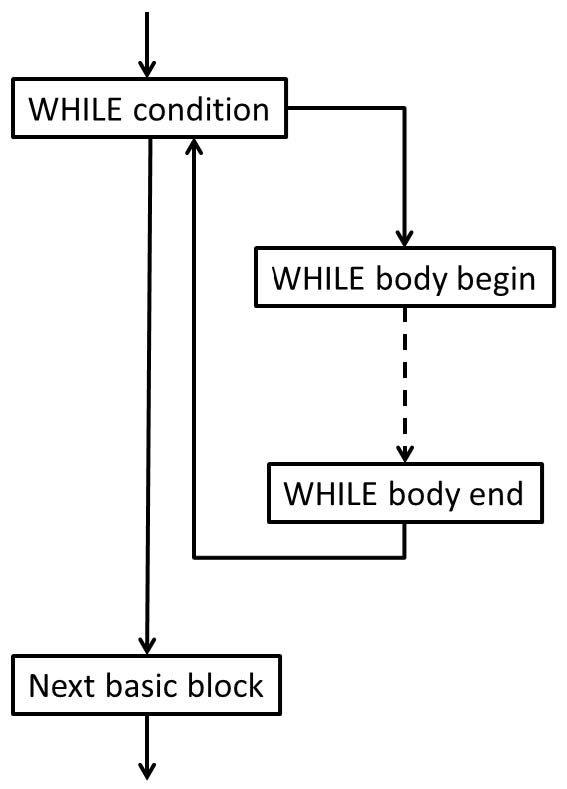
\includegraphics{content/2/chapter5/images/1.jpg}\\
图5.1 – WHILE语句的基本块
\end{center}

IR代码生成遵循这个结构。在CGProcedure类中存储一个指向当前基本块的指针,并使用llvm::IRBuilder<>的实例,将指令插入到基本块中。首先,创建基本块:\par

\begin{lstlisting}[caption={}]
void emitStmt(WhileStatement *Stmt) {
	llvm::BasicBlock *WhileCondBB = llvm::BasicBlock::Create(
		getLLVMCtx(), "while.cond", Fn);
	llvm::BasicBlock *WhileBodyBB = llvm::BasicBlock::Create(
		getLLVMCtx(), "while.body", Fn);
	llvm::BasicBlock *AfterWhileBB =
		llvm::BasicBlock::Create(
			getLLVMCtx(), "after.while", Fn);
\end{lstlisting}

Fn变量表示当前函数,getLLVMCtx()返回LLVM上下文,两者都会在之后设置。我们用一个基本块的分支来结束当前的基本块,保存条件:\par

\begin{lstlisting}[caption={}]
	Builder.CreateBr(WhileCondBB);
\end{lstlisting}

条件的基本块成为新的当前基本块。我们生成条件并以条件分支结束代码块:\par

\begin{lstlisting}[caption={}]
	setCurr(WhileCondBB);
	llvm::Value *Cond = emitExpr(Stmt->getCond());
	Builder.CreateCondBr(Cond, WhileBodyBB, AfterWhileBB);
\end{lstlisting}

接下来,生成循环体。作为最后一条指令,我们向条件的基本块添加一个分支:\par

\begin{lstlisting}[caption={}]
	setCurr(WhileBodyBB);
	emit(Stmt->getWhileStmts());
	Builder.CreateBr(WhileCondBB);
\end{lstlisting}

这就结束了WHILE语句的生成。WHILE语句后面的空基本块将成为新的当前基本块:\par

\begin{lstlisting}[caption={}]
	setCurr(AfterWhileBB);
}
\end{lstlisting}

按照这个模式,您可以为源语言的每个语句创建emit()方法。\par





















